\section{Anleitung}
Dieser Abschnitt beschreibt die Funktion sämtlicher Buttons.

\begin{figure}[H]
    \centering
    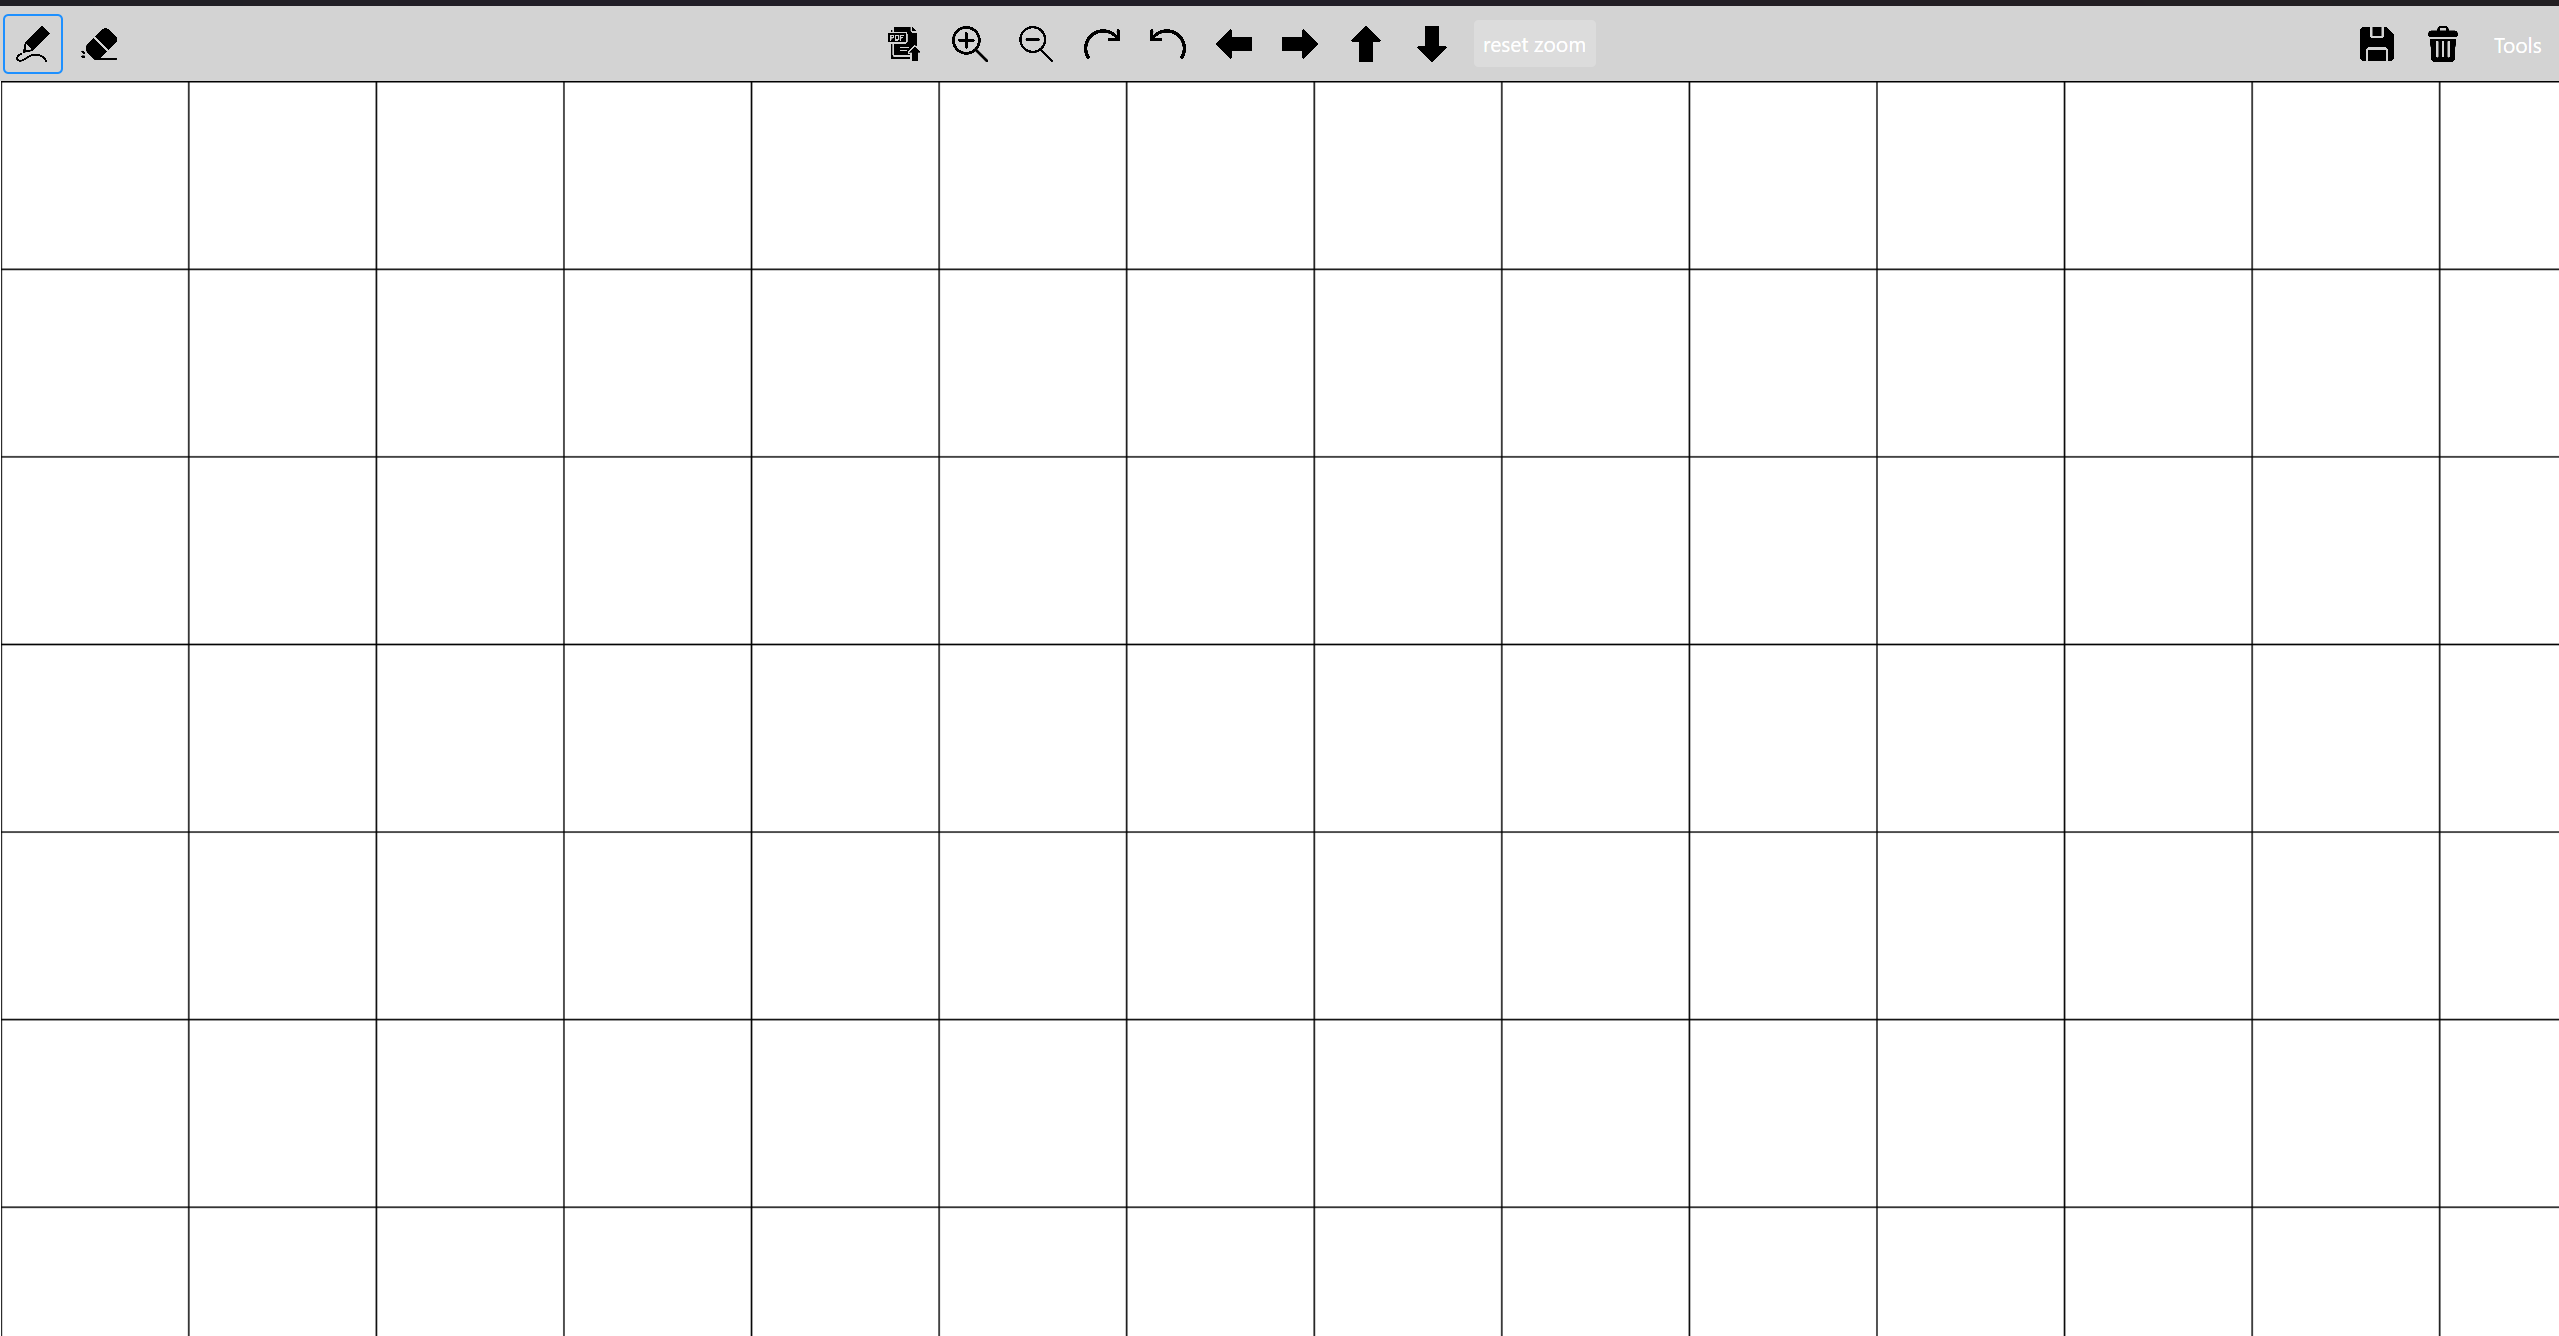
\includegraphics[width=0.5\linewidth]{graphics/ui_screenshot.png}
    \caption{Hauptansicht}
    \label{fig:ui_screenshot}
\end{figure}

Grundsätzlich sind die Funktionen wie folgt angeordnet:  
Links oben befinden sich die Werkzeuge, welche die Zeichenfunktionalität betreffen. In der Mitte sind alle Funktionen zur Steuerung der PDF-Lade- und -Anzeigeoptionen platziert. Rechts oben befinden sich die Buttons zum Löschen, Speichern sowie das Menü für Setup-Funktionen.

\subsection{Stiftfunktionen}
\begin{figure}[H]
    \centering
    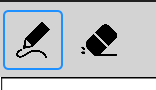
\includegraphics[width=0.5\linewidth]{graphics/stift_funktionen.png}
    \caption{Stiftfunktionen}
    \label{fig:stift_funktionen}
\end{figure}

Die Stiftfunktionen umfassen das Zeichnen sowie das Löschen an der Position des Stiftes. Der aktuell aktive Modus wird durch einen blauen Rahmen angezeigt.  
Das linke Symbol steht für den Schreibmodus mit dem Stift, während das rechte Symbol den Löschmodus aktiviert.  
Beim Anklicken des aktiven Symbols können verschiedene Optionen angepasst werden: die Strichdicke, die Radiergummigrösse sowie im Zeichenmodus zusätzlich die Stiftfarbe.

\begin{figure}[H]
    \begin{minipage}{0.48\textwidth}
        \centering
        \frame{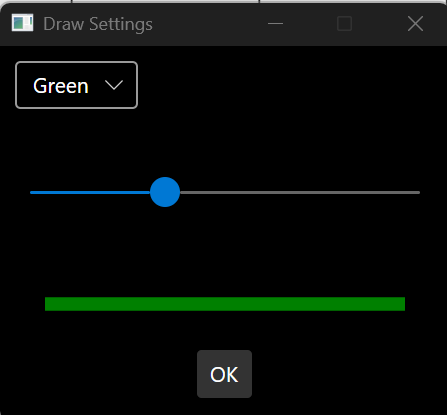
\includegraphics[width=0.9\linewidth]{graphics/draw_settings.png}}
        \caption{Zeichenmodus-Einstellungen}
        \label{fig:draw_settings}
    \end{minipage}
    \hfill
    \begin{minipage}{0.48\textwidth}
        \centering
        \frame{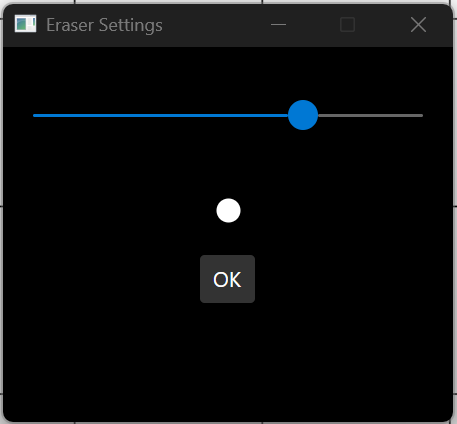
\includegraphics[width=0.9\linewidth]{graphics/eraser_settings.png}}
        \caption{Radiermodus-Einstellungen}
        \label{fig:eraser_settings}
    \end{minipage}
\end{figure}

\clearpage

\subsection{PDF-Lade- und Anzeigeoptionen}
\begin{figure}[H]
    \centering
    
\includegraphics[width=0.5\linewidth]{graphics/pdf_options.png}
    \caption{Bedienelemente für PDF-Lade- und Anzeigeoptionen}
    \label{fig:pdf_options}
\end{figure}

Die Buttons der PDF-Optionen haben – von links nach rechts – folgende Funktionen:
\begin{itemize}
    \item Öffnet den systemeigenen Dateiauswahldialog (Filepicker) und erlaubt die Auswahl eines PDF-Dokuments, das in der Zeichenfläche angezeigt werden soll.
    \item \emph{Zoom In}: Vergrössert den Inhalt der Zeichenfläche an der aktuellen Position.
    \item \emph{Zoom Out}: Verkleinert den Inhalt der Zeichenfläche an der aktuellen Position.
    \item Dreht den Inhalt der Zeichenfläche um 90° im Uhrzeigersinn.
    \item Dreht den Inhalt der Zeichenfläche um 90° gegen den Uhrzeigersinn.
    \item Bei aktivem Zoom: Verschiebt den Inhalt der Zeichenfläche nach links.
    \item Bei aktivem Zoom: Verschiebt den Inhalt der Zeichenfläche nach rechts.
    \item Bei aktivem Zoom: Verschiebt den Inhalt der Zeichenfläche nach oben.
    \item Bei aktivem Zoom: Verschiebt den Inhalt der Zeichenfläche nach unten.
    \item Setzt den Zoomfaktor sofort auf den Standardwert (0) zurück.
\end{itemize}
\section{Löschen, Speichern und Setup-Funktionen}
\begin{figure}[H]
    \centering
    
\includegraphics[width=0.5\linewidth]{graphics/setup_funktionen.png}
    \caption{Bedienelemente für Speichern, Löschen und Setup}
    \label{fig:setup_funktionen}
\end{figure}

Der Button auf der linken Seite öffnet den Datei-Explorer des Betriebssystems und erlaubt das Abspeichern des Inhalts der Zeichenfläche auf dem System.  
Der zweite Button von links löscht den gesamten Inhalt der Zeichenfläche und setzt diese auf den Zustand mit den Standardgitterlinien zurück.  
Der \emph{Tools}-Button öffnet ein Menü mit allen Funktionen rund um das Setup.

\begin{figure}[H]
    \centering
    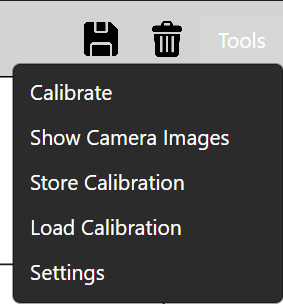
\includegraphics[width=0.5\linewidth]{graphics/toolsmenu.png}
    \caption{Tools-Menü}
    \label{fig:toolsmenu}
\end{figure}

Das Tools-Menü enthält folgende Funktionen:
\begin{itemize}
    \item \textbf{Calibrate}: Öffnet das Kalibrationsfenster, in dem nacheinander fünf rote Punkte mit dem Infrarotstift berührt werden müssen, um die Zeichenfläche zu kalibrieren.
    \begin{figure}[H]
        \centering
        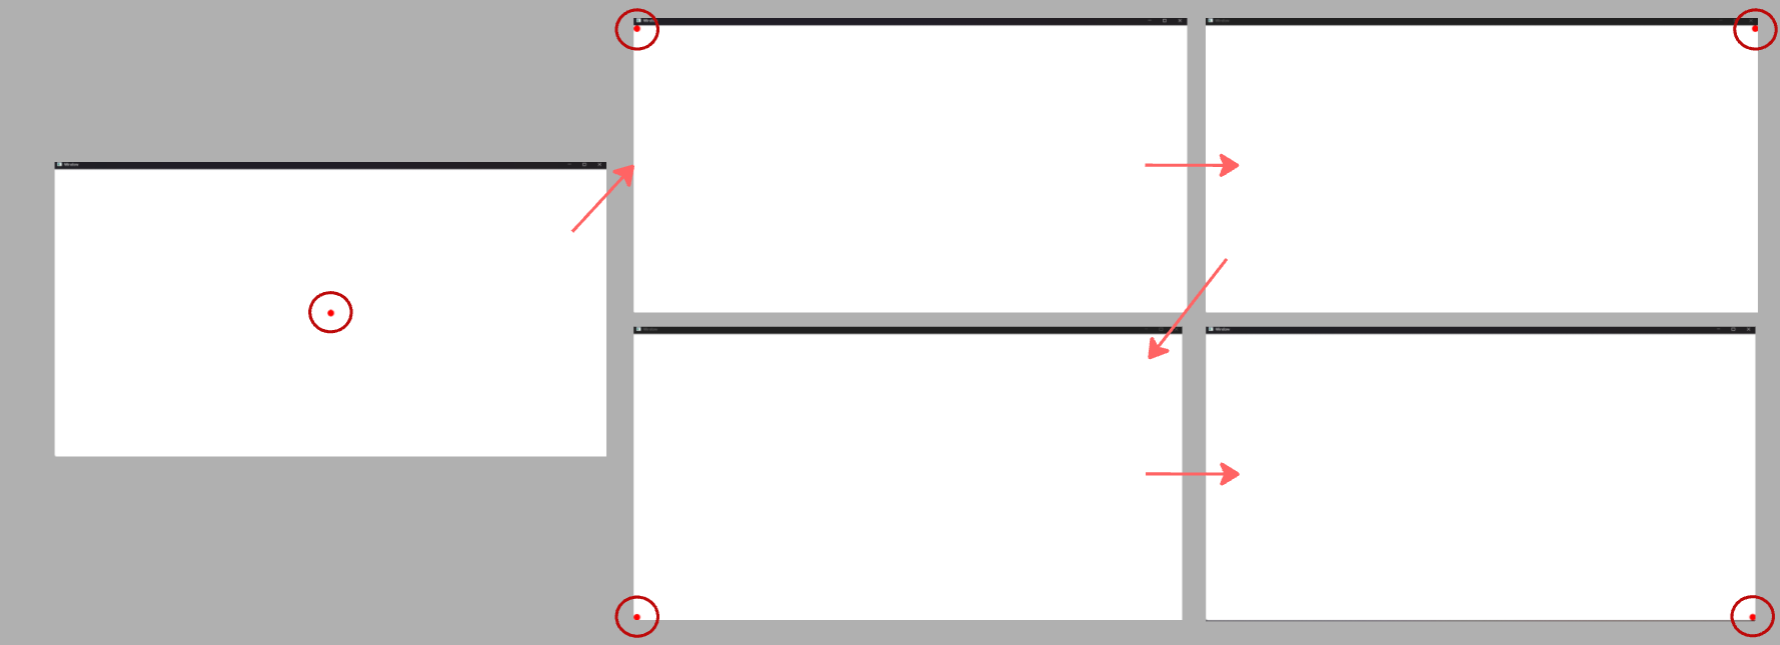
\includegraphics[width=0.5\linewidth]{graphics/ablauf_kalibration.png}
        \caption{Ablauf der Kalibration}
        \label{fig:ablauf_kalibration}
    \end{figure}
    \item \textbf{Show Camera Images}: Schaltet die Sichtbarkeit eines separaten Fensters um, in dem die Bilder der RGB- und Infrarotkamera sowie das Resultat der Binarisierung angezeigt werden.
    \item \textbf{Store Calibration}: Speichert die aktuelle Kalibration und die vorgenommenen Einstellungen.
    \item \textbf{Load Calibration}: Lädt die zuletzt gespeicherte Kalibration und Einstellungen.
    \item \textbf{Settings}: Öffnet das Einstellungsmenü.
\end{itemize}

\begin{figure}[H]
    \centering
    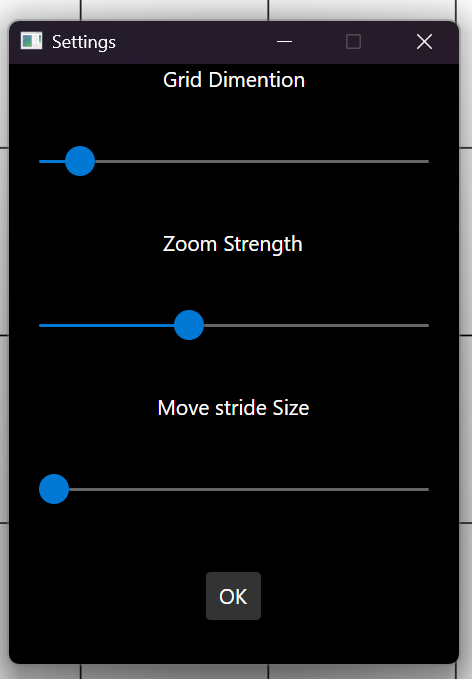
\includegraphics[width=0.5\linewidth]{graphics/settings_window.png}
    \caption{Einstellungsfenster}
    \label{fig:settings_window}
\end{figure}

Im Einstellungsmenü sind folgende Optionen verfügbar:
\begin{itemize}
    \item \textbf{Grid Dimension}: Legt die Grösse des Gitternetzes fest.
    \item \textbf{Zoom Strength}: Bestimmt, wie stark bei einem Klick hinein- oder herausgezoomt wird.
    \item \textbf{Move Stride Size}: Legt fest, um welchen Betrag der Inhalt der Zeichenfläche pro Klick verschoben wird.
\end{itemize}